\begin{figure}
	\begin{center}
		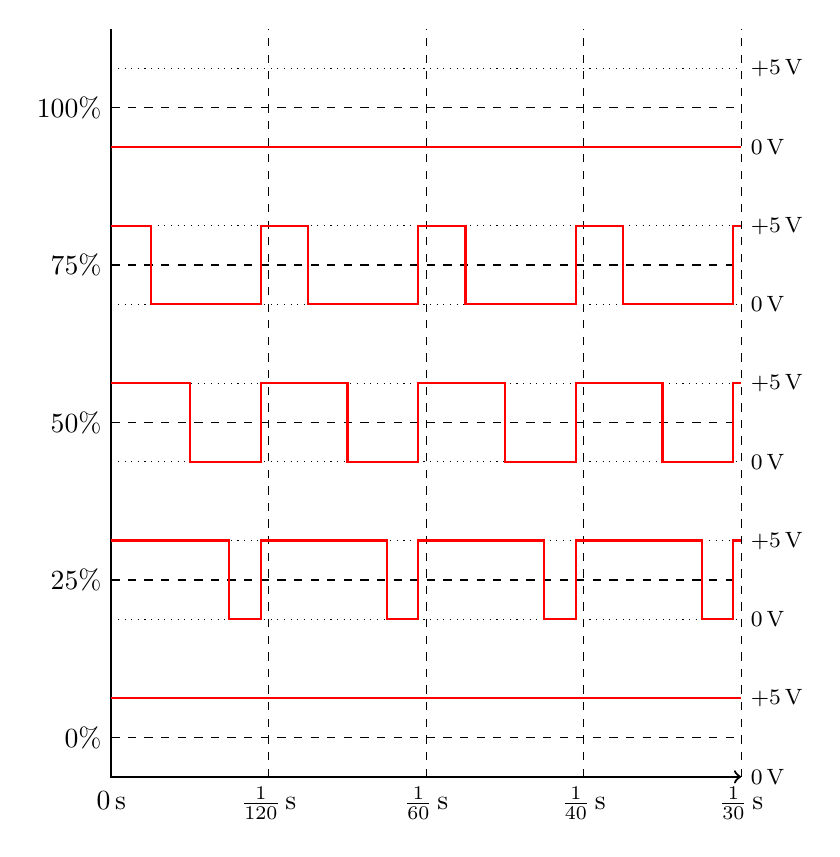
\begin{tikzpicture}[scale=.5]
			\draw [thick, <-] (16,0) -- (0,0) -- (0,19);
			\foreach \x in {4, 8, 12, 16} {
				\draw [dashed] (\x,0) -- (\x,19);
			}
			\foreach \y in {0, 4, 8, 12, 16} {
				\draw [dotted] (0,\y) -- (16,\y);
				\draw [dotted] (0,\y+2) -- (16,\y+2);
				\draw [dashed] (0,\y+1) -- (16,\y+1);
				\node [right] at (16,\y+2) {\footnotesize +5\,V};
				\node [right] at (16,\y) {\footnotesize 0\,V};
			}
			\node [left] at (0,1) {0\%};
			\node [left] at (0,5) {25\%};
			\node [left] at (0,9) {50\%};
			\node [left] at (0,13) {75\%};
			\node [left] at (0,17) {100\%};
			\node [below] at (0,0) {\vphantom{$1\over1$}0\,s};
			\node [below] at (4,0) {$1\over120$\,s};
			\node [below] at (8,0) {$1\over60$\,s};
			\node [below] at (12,0) {$1\over40$\,s};
			\node [below] at (16,0) {$1\over30$\,s};

			\draw [thick,red] (0,2) -- (16,2);
			\draw [thick,red] (0,6) -- (3,6) -- (3,4) -- (3.8,4) -- (3.8,6) --
				          (4,6) -- (7,6) -- (7,4) -- (7.8,4) -- (7.8,6) --
				          (8,6) -- (11,6) -- (11,4) -- (11.8,4) -- (11.8,6) --
				          (12,6) -- (15,6) -- (15,4) -- (15.8,4) -- (15.8,6) --
				 	  (16,6);
			\draw [thick,red] (0,10) -- (2,10) -- (2,8) -- (3.8,8) -- (3.8,10) --
				          (4,10) -- (6,10) -- (6,8) -- (7.8,8) -- (7.8,10) --
				          (8,10) -- (10,10) -- (10,8) -- (11.8,8) -- (11.8,10) --
				          (12,10) -- (14,10) -- (14,8) -- (15.8,8) -- (15.8,10) --
				 	  (16,10);
			\draw [thick,red] (0,14) -- (1,14) -- (1,12) -- (3.8,12) -- (3.8,14) --
				          (4,14) -- (5,14) -- (5,12) -- (7.8,12) -- (7.8,14) --
				          (8,14) -- (9,14) -- (9,12) -- (11.8,12) -- (11.8,14) --
				          (12,14) -- (13,14) -- (13,12) -- (15.8,12) -- (15.8,14) --
				 	  (16,14);
			\draw [thick,red] (0,16) -- (16,16);
		\end{tikzpicture}
		\caption{\label{fig:dutycycle}Duty Cycles of Channel Logic Drive Outputs}
	\end{center}
\end{figure}
